\section{Discrete Tomography}

The discrete tomography problem is the reconstruction of integral values given by a set of tomographic projections.
It specializes the conventional tomographic reconstruction problem that allows for fractional values.

\begin{definition}[Discrete Tomography]
Given an MRF $(V,E,(\mathcal{L}_v)_{v \in V},(\theta_v)_{v \in V}, (\theta_{uv})_{uv \in E})$ such that the label space is $\mathcal{L}_v = \{0,1,\ldots,K-1\}$ $\forall v \in V$ and a number of projections
$(P_i \subset V, p_i \in \N)_{i=1,\ldots,k}$ the discrete tomography problem is
\begin{equation}
\begin{array}{rl}
\min\limits_{x \in \prod_{v \in V} \mathcal{L}_v} & \sum\limits_{v \in V} \theta_v(x_v) + \sum\limits_{uv \in E} \theta_{uv}(x_u,x_v) \\
\text{s.t.}
& \sum\limits_{v \in P_i} x_v = p_i \quad \forall i \in [k]
\end{array}
\end{equation}
\end{definition}
Typically we have $\theta_v(x_i) = 0$ $\forall v \in V, x_i \in \mathcal{L}_v$, that is the unary potentials do not give any preference.

An illustration of tomographic projections is given in Figure~\ref{fig:discrete-tomo}.

\begin{figure}[H]
\begin{center}
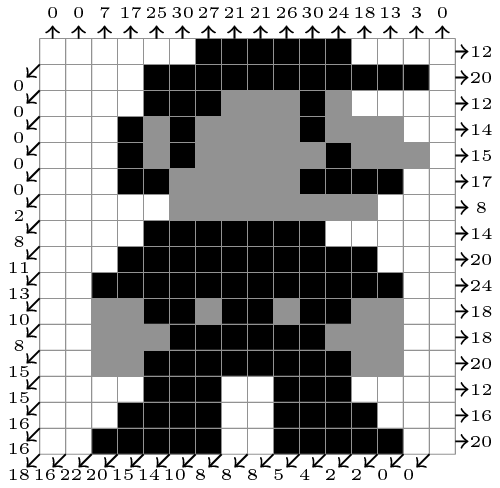
\includegraphics[width=0.7\columnwidth]{images/discrete-tomo-example.png}
\end{center}
\caption{
Exemplary discrete tomography problem.
White pixels indicate value $0$, gray ones $1$ and the black ones $2$.
Each tomographic projection is indicated by an arrow and contains those pixels $P_i$ along its ray. The numbers correspond to $p_i$.
}
\label{fig:discrete-tomo}
\end{figure}

\subsection{File Format}
We use an extension of the UAI file format used for MRFs in Section~\ref{sec:mrf-file-format}. In addition to specifying the  MRF structure the tomographic projections are appended.

\begin{fileformat}
UAI file format for MRF

PROJECTIONS
.
.
.
(*$i_1$*) + ... (*$i_{\abs{P_i}}$*) =
    (Inf,...,Inf,(*$\underbrace{0}_{p_i\text{-th place}}$*),Inf,...,Inf)
.
.
.
\end{fileformat}
for $P_i = (i_1,\ldots,i_{\abs{P_i}})$ and $i=1,\ldots,K$.

\subsection{Datasets}
\subsubsection[Synthetic Discrete Tomography]{Synthetic Discrete Tomography\footnote{\url{https://keeper.mpdl.mpg.de/f/8827141df8254eefbac4/?dl=1}}}
Around $2700$ discrete tomography instances computed from $30 \times 30$ synthetically generated images with 3 discrete intensity values and varying density of observed objects measured by varying numbers of tomographic projections.
Additionally larger discrete tomography instances of the ``Logan'' image are given.

\subsection{Algorithms}
\begin{description}[style=unboxed]
\item[Subgradient ascent on submodular MRF \& Projection~\cite{kappes2015tomogc}:]
    A binary discrete tomography solver using a Lagrange decomposition into submodular binary MRF solved with graph cuts and tomographic projection constraint solved via linear algebra.
\item[First-order optimization~\cite{zisler2016non}:]
    Combination of total variation regularized reconstruction problem with a non-convex discrete constraint optimized with forward-backward splitting.
\item[Fixed-point iteration~\cite{zisler2016discrete}:]
    Combination of a non-local projection constraint problem with a continuous convex relaxaton of the multilabeling problem solved by a fixed point iteration each of which amounts to solution of a convex auxiliary problem.
\item[Subgradient on decomposition into chain subproblems~\cite{kuske2017novel}:]
    Decompose original problems into chain subproblems that are recursively solved with fast (max,sum)-algorithms.
    The resulting Lagrange decomposition is optimized with a bundle solver.
\item[FW-Bundle Method~\cite{swoboda2019map}:]
    Similar to~\cite{kuske2017novel} but use a Frank-Wolfe based bundle method for optimization of the Lagrange decomposition.
\end{description}
